\let\negmedspace\undefined
\let\negthickspace\undefined
\documentclass[journal,12pt,onecolumn]{IEEEtran}
\usepackage{cite}
\usepackage{amsmath,amssymb,amsfonts,amsthm}
\usepackage{algorithmic}
\usepackage{graphicx}
\graphicspath{{Figs/}}
\usepackage{textcomp}
\usepackage{xcolor}
\usepackage{txfonts}
\usepackage{listings}
\usepackage{enumitem}
\usepackage{mathtools}
\usepackage{gensymb}
\usepackage{comment}
\usepackage{caption}
\usepackage[breaklinks=true]{hyperref}
\usepackage{tkz-euclide} 
\usepackage{listings}
\usepackage{gvv}                                        
%\def\inputGnumericTable{}                                 
\usepackage[latin1]{inputenc}     
\usepackage{xparse}
\usepackage{color}                                            
\usepackage{array}                                            
\usepackage{longtable}                                       
\usepackage{calc}                                             
\usepackage{multirow}
\usepackage{multicol}
\usepackage{hhline}                                           
\usepackage{ifthen}                                           
\usepackage{lscape}
\usepackage{tabularx}
\usepackage{array}
\usepackage{float}
%\newtheorem{theorem}{Theorem}[section]
%\newtheorem{theorem}{Theorem}[section]
%\newtheorem{problem}{Problem}
%\newtheorem{proposition}{Proposition}[section]
%\newtheorem{lemma}{Lemma}[section]
%\newtheorem{corollary}[theorem]{Corollary}
%\newtheorem{example}{Example}[section]
%\newtheorem{definition}[problem]{Definition}

\begin{document}


\title{4.12.7}
\author{AI25BTECH11002 - Ayush Sunil Labhade}
{\let\newpage\relax\maketitle}


\textbf{Question}:

Prove that in any ($\triangle$ ABC),
\begin{align}
\cos A = \frac{b^{2}+c^{2}-a^{2}}{2bc},
\end{align}
where (a,b,c) are the magnitudes of the sides opposite to the vertices (A,B,C) respectively.

\textbf{Solution:}

By definition of the side lengths,
\begin{align}
c &= |\vec{B} - \vec{A}|, \\
b &= |\vec{C} - \vec{A}|, \\
a &= |\vec{C} - \vec{B}|.
\end{align}

The cosine of angle \(A\) is given by
\begin{align}
\cos A &= \frac{(\vec{B} - \vec{A})^T (\vec{C} - \vec{A})}{|\vec{B} - \vec{A}| \cdot |\vec{C} - \vec{A}|} \\
       &= \frac{(\vec{B} - \vec{A})^T (\vec{C} - \vec{A})}{bc}.
\end{align}

Now, express \(a^2\) in terms of \(\vec{B} - \vec{A}\) and \(\vec{C} - \vec{A}\). Observe that
\begin{align}
\vec{C} - \vec{B} &= (\vec{C} - \vec{A}) - (\vec{B} - \vec{A}).
\end{align}
Let \(\vec{u} = \vec{C} - \vec{A}\) and \(\vec{v} = \vec{B} - \vec{A}\) for brevity. Then,
\begin{align}
\vec{C} - \vec{B} &= \vec{u} - \vec{v}.
\end{align}
Hence,
\begin{align}
a^2 &= |\vec{C} - \vec{B}|^2 \\
    &= (\vec{u} - \vec{v})^T (\vec{u} - \vec{v}) \\
    &= \vec{u}^T \vec{u} + \vec{v}^T \vec{v} - 2 \vec{u}^T \vec{v} \\
    &= b^2 + c^2 - 2 (\vec{C} - \vec{A})^T (\vec{B} - \vec{A}).
\end{align}

Rearranging,
\begin{align}
(\vec{C} - \vec{A})^T (\vec{B} - \vec{A}) &= \frac{b^2 + c^2 - a^2}{2}.
\end{align}

Substitute into the expression for \(\cos A\):
\begin{align}
\cos A &= \frac{(\vec{B} - \vec{A})^T (\vec{C} - \vec{A})}{bc} \\
       &= \frac{1}{bc} \cdot \frac{b^2 + c^2 - a^2}{2} \\
       &= \frac{b^2 + c^2 - a^2}{2bc}.
\end{align}

Thus, the required identity is proved.

		

Graph:
\begin{figure}[H]
    \centering
    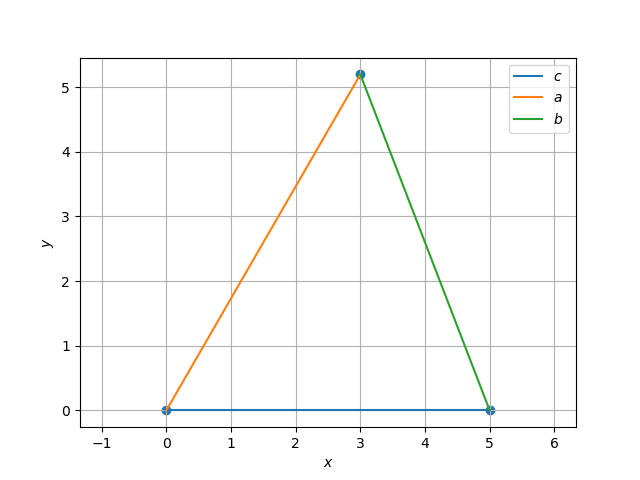
\includegraphics[scale=0.5]{plot}
    \caption{}
    \label{fig:plot}
\end{figure}
\end{document}
